\begin{center}\textbf{\color{red}LUYỆN TẬP}\\
\textbf{CHUYỂN ĐỘNG THẲNG ĐỀU - CHUYỂN ĐỘNG TỔNG HỢP\\ GIA TỐC - CHUYỂN ĐỘNG THẲNG BIẾN ĐỔI ĐỀU}
\end{center}
\setcounter{ex}{0}
\Opensolutionfile{ans}[ans/BAITAPTHEMPTCD-TN]
% ===================================================================
\begin{ex}
	Một chiếc xe ô tô xuất phát từ A lúc 6 giờ sáng, chuyển động thẳng đều tới B, cách A $\SI{180}{\kilo\meter}$. Xe tới B lúc 8 giờ 30 phút. Sau 30 phút đỗ tại B, xe chạy ngược về A với tốc độ $\SI{60}{\kilo\meter/\hour}$. Ô tô về tới A lúc
	\choice
	{$\SI{10}{\hour}$}
	{\True $\SI{12}{\hour}$}
	{$\SI{11}{\hour}$}
	{$\SI{10.5}{\hour}$}
	\loigiai{}
\end{ex}
% ===================================================================
\begin{ex}
	Một thuyền đi từ bến A đến bến B rồi lại trở về A. Biết rằng vận tốc thuyền trong nước yên lặng là $\SI{5}{\kilo\meter/\hour}$, vận tốc nước chảy là $\SI{1}{\kilo\meter/\hour}$. Vận tốc của thuyền so với bờ khi đi xuôi dòng là	
	\choice
	{$\SI{4}{\kilo\meter/\hour}$}
	{$\SI{4}{\meter/\second}$}
	{\True $\SI{6}{\kilo\meter/\hour}$}
	{$\SI{6}{\meter/\second}$}
	\loigiai{}
\end{ex}

% ===================================================================
\begin{ex}
	Đồ thị vận tốc – thời gian của một vật chuyển động như hình vẽ. Tỉ số gia tốc của vật trong thời gian OA và AB là
	\begin{center}
		\begin{tikzpicture}[scale=0.5]
			\coordinate (O) at (0,0);
			\coordinate (D) at (0,4);
			\coordinate (A) at (6.9282,0);
			\coordinate (B) at (9.2376,0);
			\coordinate (C) at (6.9282,4);
			\coordinate (t) at (10.5,0);
				\coordinate (v) at (0,5.5);
				\draw[-stealth, line width=1.5pt] (O)--(t);
				\draw[-stealth, line width=1.5pt] (O)--(v);
				\tkzMarkAngle[size=1.25cm,color=red, line width=1.5pt](A,O,C);
				\tkzLabelAngle[color=black,pos=2.25](A,O,C){$\SI{30}{\degree}$};
				\tkzMarkAngle[size=1.25cm,color=red, line width=1.5pt](C,B,A);
				\tkzMarkAngle[size=1.5cm,color=red, line width=1.5pt](C,B,A);
				\tkzLabelAngle[color=black,pos=2](C,B,A){$\SI{60}{\degree}$}
				\draw[line width=2pt, blue] (O)--(C)--(B);
				\draw[line width=1pt,dashed] (D)--(C)--(A);
				\node[left] at (D) {$40$};
				\node[below] at (t) {$\xsi{t}{\left(\second\right)}$};
				\node[above] at (v) {$v\ \left(\si{\meter/\second}\right)$};
				\node[below] at (O) {O};
				\node[below] at (A) {A};
				\node[below] at (B) {B};
		\end{tikzpicture}
	\end{center}
	\choice
	{$\dfrac{1}{3}$}
	{\True $-\dfrac{1}{3}$}
	{$3$}
	{$-3$}
	\loigiai{}
\end{ex}

% ===================================================================
\begin{ex}
	Một chất điểm chuyển động với phương trình vận tốc $v = 8 - 2t$; với ($t$ tính bằng giây và $v$ tính bằng $\si{\meter/\second}$). Thời gian chất điểm dừng lại là
	\choice
	{\True $\SI{4}{\second}$}
	{$\SI{2}{\second}$}
	{$\SI{8}{\second}$}
	{$\SI{1}{\second}$}
	\loigiai{}
\end{ex}

% ===================================================================
\begin{ex}
	Một đoàn tàu đang chạy với tốc độ $\SI{72}{\kilo\meter/\hour}$, thì hãm phanh, sau $\SI{10}{\second}$ thì dừng hẳn. Sau thời gian 4 giây, kể từ lúc hãm phanh, đoàn tàu có tốc độ là
	\choice
	{$\SI{10}{\meter/\second}$}
	{$\SI{8}{\meter/\second}$}
	{$\SI{6}{\meter/\second}$}
	{\True $\SI{12}{\meter/\second}$}
	\loigiai{}
\end{ex}
% ===================================================================
\begin{ex}
	Một chất điểm chuyển động dọc theo trục $Ox$ có phương trình tọa độ $x=4-10t$ trong đó $x$ tính theo đơn vị $\si{\kilo\meter}$ và $t$ tính theo đơn vị giờ. Quãng đường đi được của chất điểm sau 2 giờ chuyển động là
	\choice
	{$\SI{8}{\kilo\meter}$}
	{$\SI{16}{\kilo\meter}$}
	{\True $\SI{20}{\kilo\meter}$}
	{$\SI{12}{\kilo\meter}$}
	\loigiai{}
\end{ex}
% ===================================================================
\begin{ex}
	Cho đồ thị tọa độ - thời gian của một chiếc xe chuyển động thẳng như hình bên dưới. 
	\begin{center}
		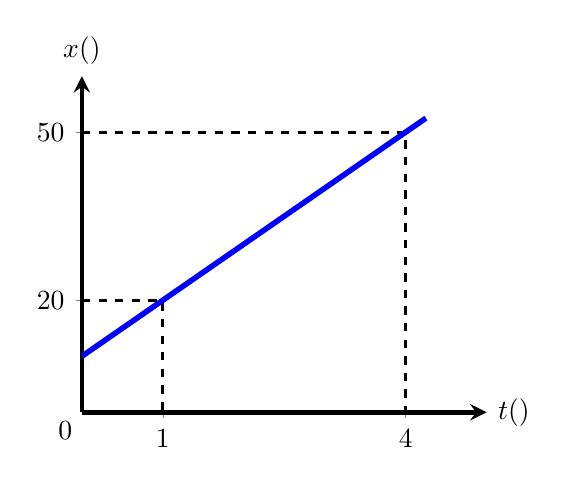
\begin{tikzpicture}  
			\begin{axis}[  ultra thick,scale=0.75,
				xmin=0,  
				xmax=5,  
				xtick={0,1,4},
				ytick={0,20,50},
				minor x tick num=0,
				minor y tick num=0,
				ymin=0,  
				ymax=60, 
				samples=300,
				axis lines=center, 
				xlabel=$\xsi{t}{\left(\si{\hour}\right)}$, 		ylabel=$\xsi{x}{\left(\si{\kilo\meter}\right)}$,
				every axis y label/.style={at=(current axis.above origin),anchor=south},  
				every axis x label/.style={at=(current axis.right of origin),anchor=west},  ]
				\draw[dashed, line width=1pt] (axis cs: 0,20)--(axis cs:1,20)--(axis cs:1,0);
				\draw[dashed, line width=1pt] (axis cs:0,50)--(axis cs:4,50)--(axis cs:4,0);
				\addplot [line width=2pt, blue, smooth, domain=0:4.25] {20+10*(x-1)};  
				\coordinate (O) at (axis cs: 0,0);
			\end{axis}  
			\node[below left] at (O) {0};
		\end{tikzpicture}
	\end{center}
	Phương trình tọa độ của xe là
	
	\choice
	{$x=15+5t$}
	{\True $x=10+10t$}
	{$x=20+10t$}
	{$x=-10+15t$}
	\loigiai{}
\end{ex}


% ===================================================================
\begin{ex}
	Một dòng sông có chiều rộng $\SI{60}{\meter}$, nước chảy với vận tốc $\SI{1}{\meter/\second}$ so với bờ. Một người lái đò chèo một chiếc thuyền đi trên sông với vận tốc $\SI{3}{\meter/\second}$ so với nước. Khi đi từ bờ này theo phương vuông góc sang bờ đối diện (điểm dự định đến). Do nước chảy nên khi sang đến bờ kia, thuyền bị trôi về phía cuối dòng. Khoảng cách từ điểm dự định đến và điểm thuyền đến thực cách nhau là
	\choice
	{$\SI{180}{\meter}$}
	{\True $\SI{20}{\meter}$}
	{$\SI{63}{\meter}$}
	{$\SI{18}{\meter}$}
	\loigiai{}
\end{ex}
% ===================================================================
\begin{ex}
Ở trên một đoạn dốc thẳng dài $\SI{130}{\meter}$, Tâm và Gia Huy đều đi xe đạp và khởi hành cùng một lúc ở hai đầu đoạn dốc. Tâm đi lên dốc với tốc độ $\SI{18}{\kilo\meter/\hour}$ và chuyển động chậm dần đều với gia tốc có độ lớn $\SI{0.2}{\meter/\second^2}$. Gia Huy đi xuống dốc với tốc độ $\SI{5.4}{\kilo\meter/\hour}$ và chuyển động nhanh dần đều với gia tốc có độ lớn $\SI{20}{\centi\meter/\second^2}$. Chọn chiều dương là chiều từ đỉnh đến chân dốc, gốc toạ độ tại đỉnh dốc, gốc thời gian là lúc hai bạn khởi hành. Phương trình chuyển động của Tâm và Gia Huy lần lượt là 
	\choice
	{$x_1=130+5t-0,1t^2\ \left(\si{\meter}, \si{\second}\right)$;  $x_2=1,5t-0,1t^2\ \left(\si{\meter}, \si{\second}\right)$}
	{$x_1=130-5t-0,1t^2\ \left(\si{\meter}, \si{\second}\right)$;  $x_2=1,5t-0,1t^2\ \left(\si{\meter}, \si{\second}\right)$}
	{$x_1=130-5t+0,1t^2\ \left(\si{\meter}, \si{\second}\right)$;  $x_2=-1,5t+0,1t^2\ \left(\si{\meter}, \si{\second}\right)$}
	{\True $x_1=130-5t+0,1t^2\ \left(\si{\meter}, \si{\second}\right)$;  $x_2=1,5t+0,1t^2\ \left(\si{\meter}, \si{\second}\right)$}
	\loigiai{}
\end{ex}

% ===================================================================
\begin{ex}
	Cùng một lúc ở hai địa điểm A, B cách nhau $\SI{300}{\meter}$, có hai xe đi ngược chiều nhau. Xe thứ nhất đi từ A với tốc độ ban đầu là $\SI{10}{\meter/\second}$ và chuyển động nhanh dần đều với gia tốc có độ lớn $\SI{2}{\meter/\second^2}$, còn xe thứ hai đi từ B với tốc độ ban đầu là $\SI{30}{\meter/\second}$ và chuyển động chậm dần đều với gia tốc có độ lớn $\SI{2}{\meter/\second^2}$. Chọn A làm gốc tọa độ, chiều dương hướng từ A đến B, gốc thời gian lúc xe thứ nhất đi qua A. Thời điểm và vị trí hai xe gặp nhau là
	\choice
	{\True $\SI{7.5}{\second}$ và $\SI{131.25}{\meter}$}
	{$\SI{10}{\second}$ và $\SI{131}{\meter}$}
	{$\SI{7.5}{\second}$ và $\SI{225}{\meter}$}
	{$\SI{15}{\second}$ và $\SI{150}{\meter}$}
	\loigiai{}
\end{ex}

\Closesolutionfile{ans}
\newpage
\begin{center}
	\textbf{BẢNG ĐÁP ÁN}
\end{center}
\inputansbox{10}{ans/BAITAPTHEMPTCD-TN}